\documentclass[../chapter_2.tex]{subfiles}
\addbibresource{../../Thesis.bib}

\begin{document}
Although not calculated often, the modeling of the aircraft's landing gear are important and should not be overlooked. However, because of the flight paths investigated in this thesis focus solely on the aircraft during flight, a simplified dynamic model is used to describe the forces and moments acting on the landing gear during landing. It should be noted that the aerodynamic calculations of the landing gear occur in the aerodynamically modeling section, while this section focuses on the moments and forces generated from the runway opposing the weight of the aircraft.

To describe the forces and moments generated during landing, a mass-spring damper system can be used in simulate the the struts, levers, and tire depression (Figure \ref{fig:ldg}) that absorb much of the forces, moments and vibrations that act onto the aircraft during landing.

\begin{figure}[!h]
        \centering
    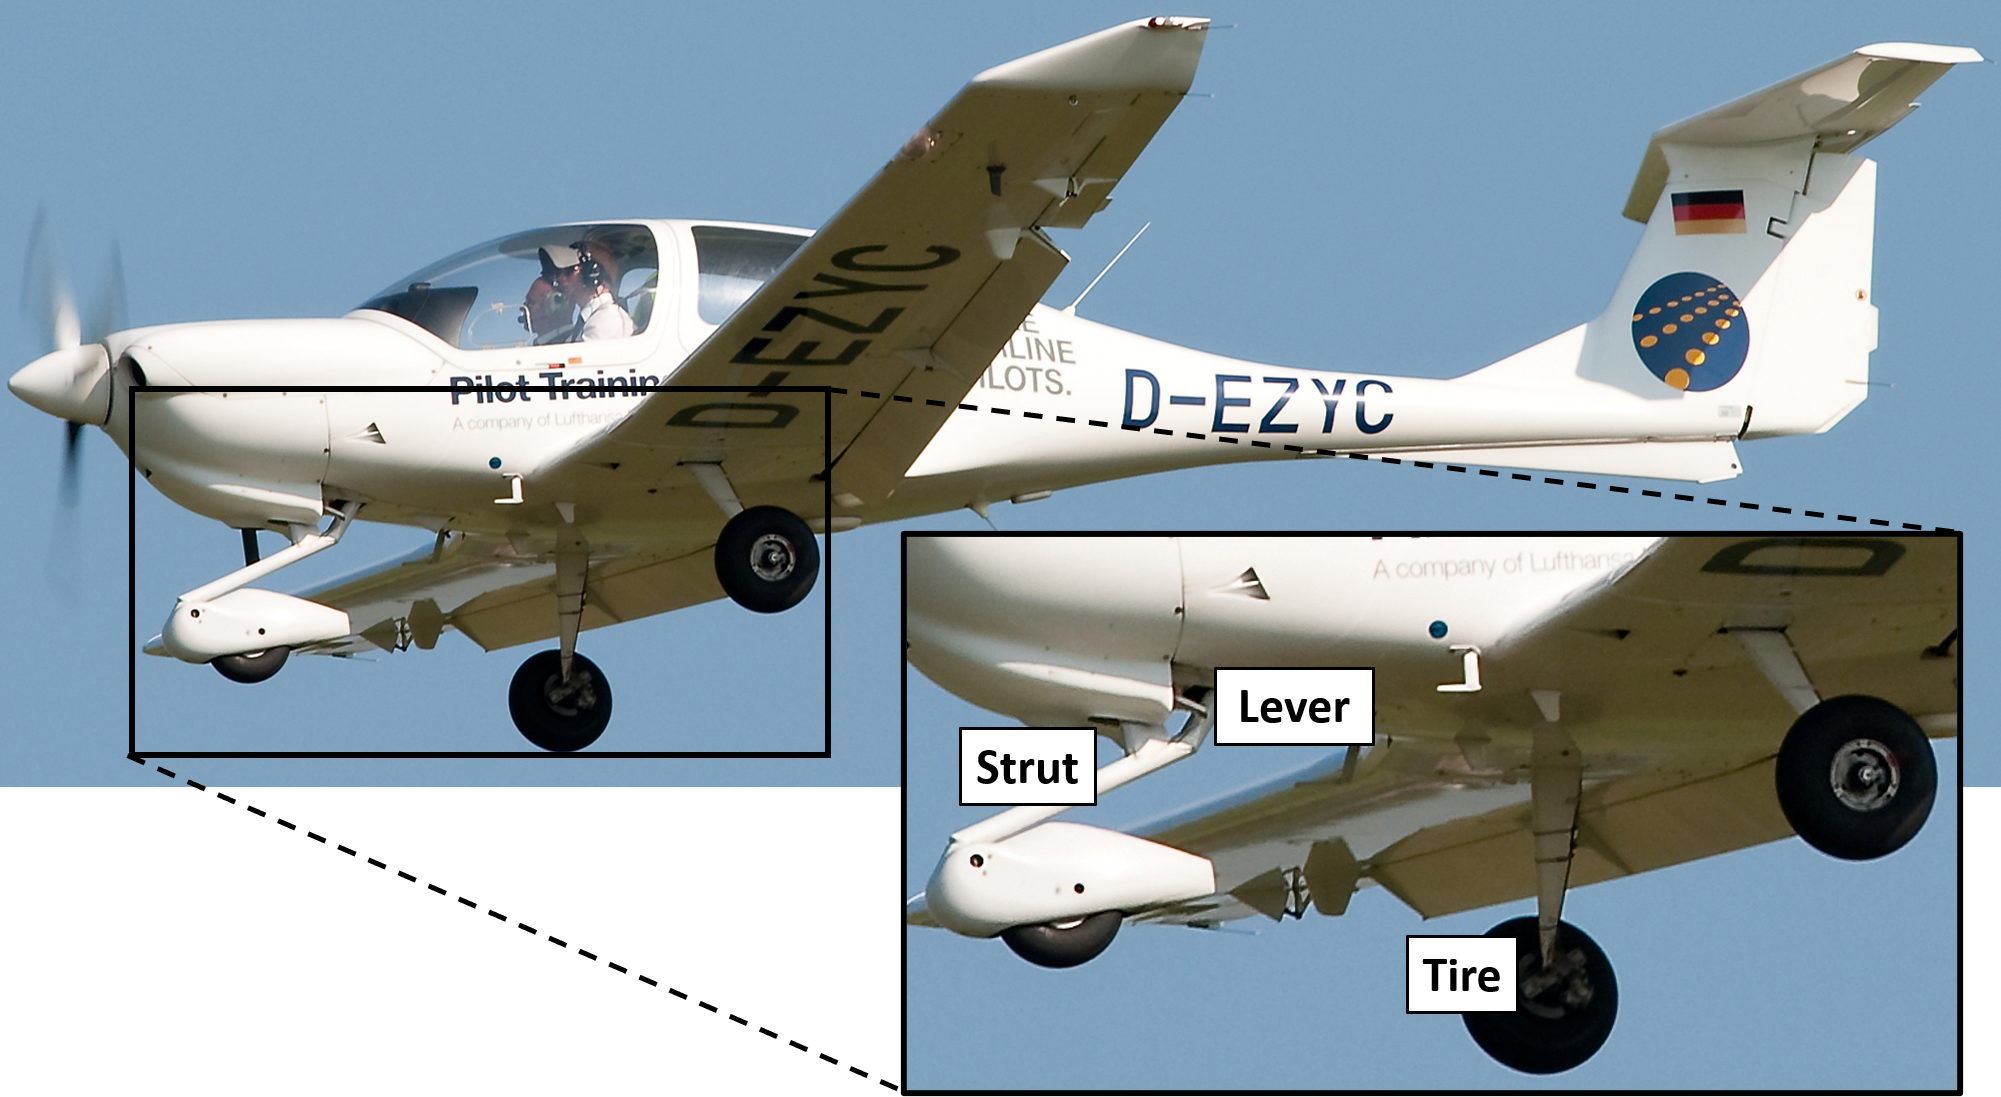
\includegraphics[width=.75\linewidth]{../../Figures/LandingGear.png}
    \caption{Identification of the landing gear components on the Diamond DA40.}
    \label{fig:ldg}
\end{figure}
\end{document}